\documentclass[11pt,twocolumn]{article}
\usepackage{caption}
\usepackage{anysize}
\usepackage{fancyhdr}
\usepackage{graphicx}
\usepackage{subcaption}
\usepackage{color}
\usepackage{balance}
\usepackage{lipsum}
\usepackage{multirow}
\usepackage{multicol}
\usepackage{booktabs}
\usepackage{pgfplots}
\usepackage{tabulary}
\usepackage{placeins}

\marginsize{.75in}{.75in}{.75in}{1in}
\pagestyle{fancy}
\rhead{\today}
\lhead{
\includegraphics[height=2.0cm]{../logo.jpg}}
\rfoot{\thepage}
\cfoot{}
\renewcommand{\headrulewidth}{0pt} %removes line from fancy header
\renewcommand{\thispagestyle}[1]{} %placers header and footer on first page 
\renewcommand{\abstractname}{Summary}
\setlength{\columnsep}{25pt}
\date{}
\title{Laboratory Gasification Memo\\Driving Force Discrimination Experiments \vspace{-6ex}}

\begin{document}

\twocolumn[
  \begin{@twocolumnfalse}
    \maketitle
    \begin{abstract}
    
In order to obtain an understanding if the main driving force for conversion of biomass to syngas is driven by kinetic or heat transfer limitations, an experimental matrix was designed to test different levels of maximum residence time and the maximum possible enthalpy change of the reactants.  Experimental results shine light on fundamental driving forces for carbon conversion and tar and methane production in the laboratory gasification system.  It was found that the total enthalpy load on the reactor was the primary driving force for carbon conversion, and lower loads led to higher conversions.  Changing residence times did not affect carbon yield or carbon release.  Finally, both residence time and enthalpy load were found to be significant factors in the production of methane and tars in the laboratory system, and some explanation is given in the text.

    \end{abstract}
  \end{@twocolumnfalse}
]

\section*{Experimental Methods}

\subsection*{Design of Experiment}

\begin{figure}
\centering
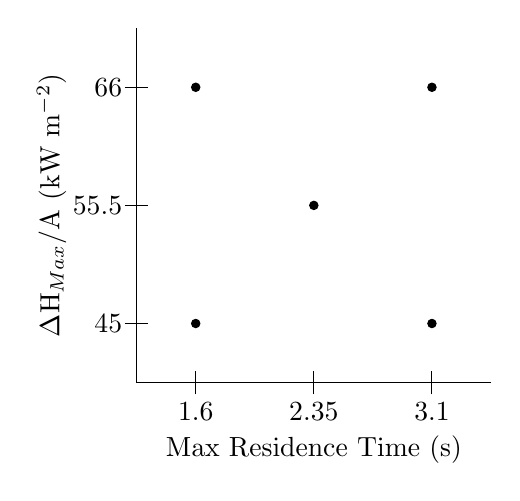
\begin{tikzpicture}[scale = 1.5]
	\draw (0,0) -- (3,0);
	\draw (0,0) -- (0,3);
	\draw (0.5,-0.1) -- (0.5,0.1) node[below = 8pt] {1.6}
		(1.5,-0.1) -- (1.5,0.1) node[below = 8pt] {2.35} node[below = 20pt]{Max Residence Time (s)}
		(2.5,-0.1) -- (2.5,0.1) node[below = 8pt] {3.1}
		(-0.1,0.5) -- (0.1,0.5) node[left = 6pt] {45}
		(-0.1,1.5) -- (0.1,1.5) node[left = 6pt] {55.5} node[xshift = -35pt, rotate = 90]{$\Delta$H$_{Max}$/A (kW m$^{-2}$)}
		(-0.1,2.5) -- (0.1,2.5) node[left = 6pt] {66};
	\filldraw [black] (0.5,0.5) circle (1pt)
		(2.5,0.5) circle (1pt)
		(1.5,1.5) circle (1pt)
		(0.5,2.5) circle (1pt)
		(2.5,2.5) circle (1pt);
\end{tikzpicture}
\caption{Two factorial experimental matrix used to vary maximum residence time and maximum $\Delta$H between experiments.}
\label{factorial}
\end{figure}

It was desired to create a two factorial matrix with a center point with the two axes representing maximum residence time (t$_{res,max}$) and maximum enthalpy change ($\Delta$H$_{max}$).  The matrix can be seen in Figure \ref{factorial}.  Partial pressure of steam and partial pressure of CO$_2$ were held constant for these experiments at 7 psi and 30 psi, respectively.  These pressures were chosen because a large number of previous gasification experiments had partial pressures of CO$_2$ and H$_2$O near these values.  

Because of the large number of possible set points in the laboratory gasifier system that would effect both the space time and maximum enthalpy simultaneously, it would have been difficult to manually design this experimental matrix.  To aid in the design, a large number of potential gasifier experiments were simulated using Sundrop Fuels' gasifier analysis software suite.  First, a flow rate of CO$_2$ was randomly assigned using a uniform distribution with a minimum possible flow rate of 3 SLPM and a maximum flow rate of 6.6 SLPM.  The partial pressure of CO$_2$ was set at 7 psi, and the appropriate flow rate of steam to lead to a partial pressure of 30 psi was found with Equation \ref{eq_steam}.

\begin{equation}
	\dot{n}_{H_2O} = \dot{n}_{CO_2} \times \frac{P_{H_2O}}{P_{CO_2}}
	\label{eq_steam}
\end{equation}

The flow rate of Argon was set at 2 SLPM for all experiments.  Biomass flow rate was randomized uniformly between 2 lbs/hr and 4 lbs/hr.  The total flow rate of entrainment gas was set to be 6 SLPM for every 1 lb/hr of biomass, which was found to be a good minimum entrainment flow rate in previous experiments using the brush feeder.  The remainder of the entrainment gas which isn't CO$_2$ was set as nitrogen.

Steam temperature was set at 500 $^\circ$C, and makeup nitrogen was uniformly randomized between 0 and 20 SLPM.  The total pressure was found using the partial pressure of steam and the total flow rate of gas into the system (Equation \ref{pressure}).  The maximum residence time and the maximum enthalpy change were calculated for each simulated run using Sundrop Fuel's gasifier analysis software.  Experiments which could not be run due to system limitations were removed from the potential runs, and enthalpy and maximum residence time targets were chosen to maximize the change in each measure.  Set points for all experiments are outlined in Appendix \ref{app_experiments}.

\begin{equation}
	P_{tot} = P_{H_2O} \times \frac{\dot{n}_{tot}}{\dot{n}_{H_2O}}
	\label{pressure}
\end{equation}

%%%%%%%%%%%%%%%%%
%%%%%%%%%%%%%%%%%

\subsection*{Calculations}

Two measures of carbon conversion are discussed in this memo.  The first is the fraction of carbon in the biomass which is converted to either CO or CO$_2$, as these are the two species which are the precursor to synthetic liquid products in the planned commercial process.  This measure is refered to as carbon yield, although it has been referred to in the past as good conversion, and is given in Equation \ref{eq_c_yield}.

\begin{equation}
	Y_{CO+CO_2} = \frac{\dot{n}_{CO,out}+\dot{n}_{CO_2,out} - \dot{n}_{CO_2,in}}{\dot{n}_{C_{biomass},in}}
	\label{eq_c_yield}
\end{equation}

The second measure is carbon release, which has been referred to in the past as total conversion.  This was calculated using Equation \ref{eq_c_release} and is a representation of the fraction of carbon in the biomass which is converted to any gaseous specie detected by the mass spectrometer.

\begin{equation}
	X_{C} = \frac{\dot{n}_{C_{gas},out}- \dot{n}_{CO_2,in}}{\dot{n}_{C_{biomass},in}}
	\label{eq_c_release}
\end{equation}

Tar loading is a measure of the mass of tars detected by the mass spectrometer (C$_6$H$_6$, C$_7$H$_8$, and C$_{10}$H$_8$) in a standard volume of product gas.  This value was calculated using Equation \ref{eq_tar}.

\begin{equation}
	C_{tar} = \frac{\dot{m}_{C_6H_6}+\dot{m}_{C_7H_8} + \dot{m}_{C_{10}H_8}}{\dot{V}(\frac{P}{P_{std}})(\frac{T_{std}}{T})}
	\label{eq_tar}
\end{equation}

Finally, the last measure discussed in this memo is methane yield.  It is a representation of the fraction of carbon in the biomass which is converted to methane, and it was calculated using Equation \ref{eq_ch4}.  A table defining all variables used in this memo can be found in Appendix \ref{app_var}.

\begin{equation}
	Y_{CH_4} = \frac{\dot{n}_{CH_4}}{\dot{n}_{C_{biomass},in}}
	\label{eq_ch4}
\end{equation}

%%%%%%%%%%%%%%%%%
%%%%%%%%%%%%%%%%%

\section*{Results and Discussion}

Because only inlet conditions of the reactants were needed to calculate the maximum residence time, the experimental matrix was designed based on this calculation.  Once experiments were completed and outlet conditions were known, a minimum residence time could be calculated assuming all products reached the wall temperature of the reactor and reacted fully immediately upon entering the reactor.  In reality, the actual residence time  was somewhere between these boundaries, and the actual residence time would be very difficult to estimate with the data known from the experiments.  

Plotted results are shown in Appendices \ref{app_plots_cyield}, \ref{app_plots_crel}, \ref{app_plots_tar}, and \ref{app_plots_ch4} for carbon yield, carbon release, tar loading, and methane yield using both the maximum and minimum residence times for visualization purposes.  ANOVA results are shown using only minimum residence time.  While the magnitude of the effects may be slightly different when using either minimum or maximum residence time, the time chosen for analysis does not change which factors are shown to be statistically significant when using ANOVA.

%%%%%%%%%%%%%%%%%
%%%%%%%%%%%%%%%%%

\subsection*{Carbon Yield}

Carbon yield results are plotted in Figures \ref{maxrt_vs_cyield}, \ref{minrt_vs_cyield}, \ref{dh_vs_cyield_maxrt}, and \ref{dh_vs_cyield_minrt} in Appendix \ref{app_plots_cyield}.  ANOVA results are given in Table \ref{anova_cyield}, and factors which had a statistically significant effect on carbon yield are highlighted in red.  At 1350 $^\circ$C, minimum residence time was not statistically significant while $\Delta H_{Max}$/A was.  Both minimum residence time and $\Delta H_{Max}$/A were statistically signficant at 1450 $^\circ$C.  However, as shown in the aforementioned plots, higher residence times led to lower carbon yields, if there was an effect.  Since it is very unlikely that the reaction would proceed backwards and lead to lower conversions at longer residence times, it's likely that the effect did not exist, or that another factor was correlated with the changing residence times that is causing the difference in calculated carbon yields.  Further tests may be held in the future holding different factors constant to see what is actually driving the variance.

\begin{table}
	\centering
	\caption{ANOVA results on effects of designed experimental campaign for carbon yield.}
	\begin{tabular}{r c c}
		\toprule
		\multicolumn{1}{c}{\multirow{2}{*}{Effect}}		& 	\multicolumn{2}{c}{Prob \textless F	}	\\
		{}								&	1350 $^\circ$C					&	1450 $^\circ$C			\\
		\midrule
		t$_{res,min}$						&	0.1845						&	\textcolor{red}{0.0059}	\\
		$\Delta H_{Max}$/A					&	\textcolor{red}{\textless 0.0001}	&	\textcolor{red}{0.0002}	\\
		t$_{res,min}\times \Delta H_{Max}$/A	&	0.5060						&	0.9646				\\
		\bottomrule
	\end{tabular}
	\label{anova_cyield}
\end{table}

%%%%%%%%%%%%%%%%%
%%%%%%%%%%%%%%%%%

\subsection*{Carbon Release}

Carbon release results are plotted in Figures \ref{maxrt_vs_crel}, \ref{minrt_vs_crel}, \ref{dh_vs_crel_maxrt}, and \ref{dh_vs_crel_minrt} in Appendix \ref{app_plots_crel}.  Results from ANOVA, shown in Table \ref{anova_crel} reflected what was seen in carbon yield measurements.  The total maximum enthalpy load was a significant factor in the carbon release at both 1450 $^\circ$C and 1350 $^\circ$C.  Again, while minimum residence time was statistically significant at 1450 $^\circ$C, longer residence times actually gave lower conversions.  Since this result contradicts kinetic considerations, further tests may be completed in the future to see if some other factor correlated with the changing residence times was causing the apparent dependency of conversion on residence time.

\begin{table}
	\centering
	\caption{ANOVA results on effects of designed experimental campaign for carbon release.}
	\begin{tabular}{r c c}
		\toprule
		\multicolumn{1}{c}{\multirow{2}{*}{Effect}}		& 	\multicolumn{2}{c}{Prob \textless F	}	\\
		{}								&	1350 $^\circ$C			&	1450 $^\circ$C			\\
		\midrule
		t$_{res,min}$						&	0.1175				&	\textcolor{red}{0.0017}	\\
		$\Delta H_{Max}$/A					&	\textcolor{red}{0.0005}	&	\textcolor{red}{0.0002}	\\
		t$_{res,min}\times \Delta H_{Max}$/A	&	0.8289				&	0.7615				\\
		\bottomrule
	\end{tabular}
	\label{anova_crel}
\end{table}

%%%%%%%%%%%%%%%%%
%%%%%%%%%%%%%%%%%

\subsection*{Tar Loading}

Figures \ref{maxrt_vs_tar}, \ref{minrt_vs_tar}, \ref{dh_vs_tar_maxrt}, and \ref{dh_vs_tar_minrt} in Appendix \ref{app_plots_tar} show the results for tar loading values from each experiment in the campaign.  Longer residence times and lower enthalpy loads appear to have led to lower tars at 1350 $^\circ$C.  ANOVA results shown in Table \ref{anova_tar} show that both residence time and $\Delta H_{Max}$/A had statistically significant effects on the amount of tars produced at 1350 $^\circ$C, but not at 1450 $^\circ$C.  This is similar to past results at 1450 $^\circ$C where the tar levels were on the same order of magnitude as the variance between runs, so conclusions about difference in tar levels cannot be made.

\begin{table}
	\centering
	\caption{ANOVA results on effects of designed experimental campaign for tar loading.}
	\begin{tabular}{r c c}
		\toprule
		\multicolumn{1}{c}{\multirow{2}{*}{Effect}}		& 	\multicolumn{2}{c}{Prob \textless F	}	\\
		{}								&	1350 $^\circ$C	&	1450 $^\circ$C			\\
		\midrule
		t$_{res,min}$						&	\textcolor{red}{\textless 0.0001}	&	0.0654			\\
		$\Delta H_{Max}$/A					&	\textcolor{red}{0.0015}			&	0.8029			\\
		t$_{res,min}\times \Delta H_{Max}$/A	&	\textcolor{red}{0.0002}			&	0.2309			\\
		\bottomrule
	\end{tabular}
	\label{anova_tar}
\end{table}

It is important to note that residence time had a significant effect on tar loading at 1350 $^\circ$C, but it did not have a significant effect on conversion measures at this temperature.  It is possible that the actual temperature of the gaseous products leaving the reactor was at a temperature where there were still some kinetic limitations on tar cracking reactions, but the temperature was high enough where the primary solids pyrolysis reactions happened extremely quickly.  Increasing the heat transfer to the reactants, especially at the bottom of the reactor where fewer solids exist to efficiently transfer radiation energy from the walls of the reactor, may increase the outlet gas temperature to a point where these cracking reactions proceed extremely quickly and the dependence in residence time may vanish.

%%%%%%%%%%%%%%%%%
%%%%%%%%%%%%%%%%%

\subsection*{Methane Yield}

Methane yield showed similar results as tar loading.  Results are shown in Figures \ref{maxrt_vs_ch4}, \ref{minrt_vs_ch4}, \ref{dh_vs_ch4_maxrt}, and \ref{dh_vs_ch4_minrt} in Appendix \ref{app_plots_ch4}.  ANOVA results, shown in Table \ref{anova_ch4}, show that both residence time and $\Delta H_{Max}$/A were statistically significant for methane yield at 1350  $^\circ$C as well as 1450  $^\circ$C.  Longer space times and lower enthalpy loads led to lower methane yields at both temperatures.

\begin{table}
	\centering
	\caption{ANOVA results on effects of designed experimental campaign for methane yield.}
	\begin{tabular}{r c c}
		\toprule
		\multicolumn{1}{c}{\multirow{2}{*}{Effect}}		& 	\multicolumn{2}{c}{Prob \textless F	}	\\
		{}								&	1350 $^\circ$C	&	1450 $^\circ$C			\\
		\midrule
		t$_{res,min}$						&	\textcolor{red}{\textless 0.0001}	&	\textcolor{red}{0.0001}	\\
		$\Delta H_{Max}$/A					&	\textcolor{red}{\textless 0.0001}	&	\textcolor{red}{0.0065}	\\
		t$_{res,min}\times \Delta H_{Max}$/A	&	\textcolor{red}{0.0009}			&	0.1305				\\
		\bottomrule
	\end{tabular}
	\label{anova_ch4}
\end{table}
 
Like with tar loading, it's possible that the temperatures that the product gases were reaching were still at a low enough temperature where methane reforming was kinetically limited.  Increasing heat transfer in the reactor to the gas phase near the exit may raise the temperature of these gases to a point where methane reforming happens very rapidly and the dependency on space time may go away.  Further tests will need to be completed in the future to see if this is the case.

\subsection*{Normalized Heat Duty}

One good test to see if the carbon conversions are driven by heat transfer is to normalize the heat duty by dividing it by the temperature of the reactor wall to the fourth power.  Since previous heat transfer tests have shown that the actual wall temperature is about 50 $^\circ$C lower than what is measured by the skin thermocouples during normal operation, the temperatures were lowered by 50 $^\circ$C.  Graphs showing carbon yield and carbon release plotted against this normalized heat duty are found in Appendix \ref{app_norm} in Figures \ref{normalized_cyield} and \ref{normalized_crel}.

%%%%%%%%%%%%%%%%%
%%%%%%%%%%%%%%%%%

\balance
\section*{Conclusion}

Experiments showed that residence time did not have an effect on carbon conversion.  While residence time showed a statistically significant effect on carbon yield and carbon release at 1450 $^\circ$C, the effect is opposite of what has been observed in the past and may be due to another untested factor correlated with residence time in the experimental design.  There was no statistically significant effect of residence time on either measure of conversion at 1350 $^\circ$C.  Heat duty, on the other hand, had a significant effect on carbon conversion at both temperatures.

Residence time did, however, have an effect on tar loading at 1350 $^\circ$C and methane yield at both 1350 $^\circ$C and 1450 $^\circ$C.  Longer times led to lower amount of the undesired products.  Effects that enthalpy load had on tar and methane production mirrored those displayed by residence time.

Future experiments should be completed which will hold different factors constant throughout the experimental campaign.  Additionally, the conversions seen for given enthalpy loads are lower than previous gasification experiments.  The biomass used in these experiments is from a different production run.  Experiments will be completed in the near future that repeat previous experimental set points with the new biomass to compare the results with old biomass.  If results come back with different conversions, then old biomass will be used under the same conditions to see if there has been a change in the system recently.

\onecolumn
\newpage
\appendix

%%%%%%%%%%%%%%%%%
%%%%%%%%%%%%%%%%%

\section{Carbon Yield Plots}
\label{app_plots_cyield}


\begin{minipage}{\textwidth}
\centering
% Maximum Residence Time vs X_good Colored by dH_max %
	\begin{tikzpicture}
	\begin{axis} [scale = .9,
		title =  1450 $^\circ$C,
		xlabel = Maximum Residence Time (s), 
		ylabel= Carbon Yield,
		yticklabel style = {/pgf/number format/.cd,fixed zerofill}, 
		xticklabel style = {/pgf/number format/.cd,fixed zerofill,precision=1}, 
		colorbar horizontal, 
		colorbar style = {
			at={(1.15,-.35)},anchor=north,
			xticklabel style = {/pgf/number format/.cd,fixed zerofill,precision=0}, 
			xlabel=$\Delta$H$_{Max}$/A (kW m$^{-2}$),
			xlabel style = {yshift = 1.7cm},
			point meta min = 45}
]
	\addplot[
		scatter, 
		only marks, 
		scatter src = explicit,] 
		table [
			col sep = comma,
			x = space_time_avg, 
			y = X_good_avg, 
			meta = dH/A]  
	{enthalpy_runs_1450.csv};
	\end{axis}
	\begin{axis} [scale = .9, at={(7.5cm,0)},
		title =  1350 $^\circ$C,
		xlabel = Maximum Residence Time (s), 
		yticklabel style = {/pgf/number format/.cd,fixed zerofill}, 
		xticklabel style = {/pgf/number format/.cd,fixed zerofill,precision=1}]
	\addplot[
		scatter, 
		only marks, 
		scatter src = explicit,] 
		table [
			col sep = comma,
			x = space_time_avg, 
			y = X_good_avg, 
			meta = dH/A]  
	{enthalpy_runs_1350.csv};
	\end{axis}

	\end{tikzpicture}
	\captionof{figure}{Results for carbon yield plotted against maximum residence time and colored by enthalpy load.  At 1450 $^\circ$C, longer space times actually lead to lower conversions for similar enthalpy loads. At 1350 $^\circ$C, the difference in conversions at different space times but similar enthalpy loads is close to the variance between replicates, and ANOVA results show that residence time has no effect on carbon yield.}
	\label{maxrt_vs_cyield}
\end{minipage}


\begin{minipage}{\textwidth}
\centering
% Minimum Residence Time vs X_good Colored by dH_max %
	\begin{tikzpicture}
	\begin{axis} [scale = .9,
		title =  1450 $^\circ$C,
		xlabel = Minimum Residence Time (s), 
		ylabel= Carbon Yield,
		yticklabel style = {/pgf/number format/.cd,fixed zerofill}, 
		xticklabel style = {/pgf/number format/.cd,fixed zerofill,precision=2}, 
		colorbar horizontal, 
		colorbar style = {
			at={(1.15,-.35)},anchor=north,
			xticklabel style = {/pgf/number format/.cd,fixed zerofill,precision=0}, 
			xlabel=$\Delta$H$_{Max}$/A (kW m$^{-2}$), 
			xlabel style = {yshift = 1.7cm},
			point meta min = 45}
]
	\addplot[
		scatter, 
		only marks, 
		scatter src = explicit,] 
		table [
			col sep = comma,
			x = tau_min, 
			y = X_good_avg, 
			meta = dH/A]  
	{enthalpy_runs_1450.csv};
	\end{axis}
	\begin{axis} [scale = .9, at={(7.5cm,0)},
		title =  1350 $^\circ$C,
		xlabel = Minimum Residence Time (s), 
		yticklabel style = {/pgf/number format/.cd,fixed zerofill}, 
		xticklabel style = {/pgf/number format/.cd,fixed zerofill,precision=2}, 
		xtick = {.3,.4,.5,.6}
]
	\addplot[
		scatter, 
		only marks, 
		scatter src = explicit,] 
		table [
			col sep = comma,
			x = tau_min, 
			y = X_good_avg, 
			meta = dH/A]  
	{enthalpy_runs_1350.csv};
	\end{axis}
	\end{tikzpicture}
	\captionof{figure}{Carbon yield is plotted against minimum residence time rather than maximum residence time.  Although data points are shifted across the x-axis relative to each other, the same conclusions are reached when looking at minimum residence time rather than maximum residence time.}
	\label{minrt_vs_cyield}
\end{minipage}


\begin{minipage}{\textwidth}
\centering
% dH/A vs X_good Colored by space_time %
	\begin{tikzpicture}
	\begin{axis} [scale = .9,
		title =  1450 $^\circ$C,
		xlabel = $\Delta$H$_{Max}$/A (kW m$^{-2}$), 
		ylabel= Carbon Yield,
		yticklabel style = {/pgf/number format/.cd,fixed zerofill}, 
		xticklabel style = {/pgf/number format/.cd,fixed zerofill,precision=0}, 
		colorbar horizontal, 
		colorbar style = {
			at={(1.15,-.35)},anchor=north,
			xticklabel style = {/pgf/number format/.cd,fixed zerofill,precision=1}, 
			xlabel=Maximum Residence Time (s), 
			xlabel style = {yshift = 1.7cm},
			xtick = {1.5,2.3,3.0},
			point meta min = 1.4
}
]
	\addplot[
		scatter, 
		only marks, 
		scatter src = explicit,] 
		table [
			col sep = comma,
			x = dH/A, 
			y = X_good_avg, 
			meta = space_time_avg]  
	{enthalpy_runs_1450.csv};
	\end{axis}
	\begin{axis} [scale = .9, at={(7.5cm,0)},
		title =  1350 $^\circ$C,
		xlabel = $\Delta$H$_{Max}$/A (kW m$^{-2}$), 
		yticklabel style = {/pgf/number format/.cd,fixed zerofill}, 
		xticklabel style = {/pgf/number format/.cd,fixed zerofill,precision=0}, 
]
	\addplot[
		scatter, 
		only marks, 
		scatter src = explicit,] 
		table [
			col sep = comma,
			x = dH/A, 
			y = X_good_avg, 
			meta = space_time_avg]  
	{enthalpy_runs_1350.csv};
	\end{axis}
	\end{tikzpicture}
	\captionof{figure}{Here, carbon yield is plotted against $\Delta$H$_{Max}$/A.  At 1450 $^\circ$C, it appears as though lower residence times lead to higher conversions, which is counter-intuitive.  At 1350 $^\circ$C, the conversions at different  residence times collapse onto each other, and it is easy to see the lack of effect that residence time has on carbon yield.}
	\label{dh_vs_cyield_maxrt}
\end{minipage}


\begin{minipage}{\textwidth}
\centering
% dH/A vs X_good Colored by minimum residence time %
	\begin{tikzpicture}
	\begin{axis} [scale = .9,
		title =  1450 $^\circ$C,
		xlabel = $\Delta$H$_{Max}$/A (kW m$^{-2}$), 
		ylabel= Carbon Yield,
		yticklabel style = {/pgf/number format/.cd,fixed zerofill}, 
		xticklabel style = {/pgf/number format/.cd,fixed zerofill,precision=0}, 
		colorbar horizontal, 
		colorbar style = {
			at={(1.15,-.35)},anchor=north,
			xticklabel style = {/pgf/number format/.cd,fixed zerofill,precision=2}, 
			xlabel=Minimum Residence Time (s), 
			xlabel style = {yshift = 1.7cm}
}
]
	\addplot[
		scatter, 
		only marks, 
		scatter src = explicit,] 
		table [
			col sep = comma,
			x = dH/A, 
			y = X_good_avg, 
			meta = tau_min]  
	{enthalpy_runs_1450.csv};
	\end{axis}
	\begin{axis} [scale = .9, at={(7.5cm,0)},
		title =  1350 $^\circ$C,
		xlabel = $\Delta$H$_{Max}$/A (kW m$^{-2}$), 
		yticklabel style = {/pgf/number format/.cd,fixed zerofill}, 
		xticklabel style = {/pgf/number format/.cd,fixed zerofill,precision=1}, 
]
	\addplot[
		scatter, 
		only marks, 
		scatter src = explicit,] 
		table [
			col sep = comma,
			x = dH/A, 
			y = X_good_avg, 
			meta = tau_min]  
	{enthalpy_runs_1350.csv};
	\end{axis}
	\end{tikzpicture}
	\captionof{figure}{Carbon yield is plotted against $\Delta$H$_{Max}$/A and colored according to minimum residence time.  Again, the same conclusions are met no matter if minimum or maximum residence time is used for analysis. }
	\label{dh_vs_cyield_minrt}
\end{minipage}

%%%%%%%%%%%%%%%%%
%%%%%%%%%%%%%%%%%

\section{Carbon Release Plots}
\label{app_plots_crel}


\begin{minipage}{\textwidth}
\centering
% Maximum Residence Time vs X_tot Colored by dH_max %
	\begin{tikzpicture}
	\begin{axis} [scale = .9,
		title =  1450 $^\circ$C,
		xlabel = Maximum Residence Time (s), 
		ylabel= Carbon Release,
		yticklabel style = {/pgf/number format/.cd,fixed zerofill}, 
		xticklabel style = {/pgf/number format/.cd,fixed zerofill,precision=1}, 
		colorbar horizontal, 
		colorbar style = {
			at={(1.15,-.35)},anchor=north,
			xticklabel style = {/pgf/number format/.cd,fixed zerofill,precision=0}, 
			xlabel=$\Delta$H$_{Max}$/A (kW m$^{-2}$), 
			xlabel style = {yshift = 1.7cm},
			point meta min = 45}
]
	\addplot[
		scatter, 
		only marks, 
		scatter src = explicit,] 
		table [
			col sep = comma,
			x = space_time_avg, 
			y = X_tot_avg, 
			meta = dH/A]  
	{enthalpy_runs_1450.csv};
	\end{axis}
	\begin{axis} [scale = .9, at={(7.5cm,0)},
		title =  1350 $^\circ$C,
		xlabel = Maximum Residence Time (s), 
		yticklabel style = {/pgf/number format/.cd,fixed zerofill}, 
		xticklabel style = {/pgf/number format/.cd,fixed zerofill,precision=1}]
	\addplot[
		scatter, 
		only marks, 
		scatter src = explicit,] 
		table [
			col sep = comma,
			x = space_time_avg, 
			y = X_tot_avg, 
			meta = dH/A]  
	{enthalpy_runs_1350.csv};
	\end{axis}

	\end{tikzpicture}
	\captionof{figure}{Carbon release results show the same trends as carbon yield, but the difference in carbon release for similar residence times and different enthalpy loads are slightly larger than they were for carbon yield.  At 1450 $^\circ$C, maximum residence time shows a negative effect on conversion and has no effect on conversion at 1350 $^\circ$C.}
	\label{maxrt_vs_crel}
\end{minipage}


\begin{minipage}{\textwidth}
\centering
% Minimum Residence Time vs X_tot Colored by dH_max %
	\begin{tikzpicture}
	\begin{axis} [scale = .9,
		title =  1450 $^\circ$C,
		xlabel = Minimum Residence Time (s), 
		ylabel= Carbon Release,
		yticklabel style = {/pgf/number format/.cd,fixed zerofill}, 
		xticklabel style = {/pgf/number format/.cd,fixed zerofill,precision=2}, 
		colorbar horizontal, 
		colorbar style = {
			at={(1.15,-.35)},anchor=north,
			xticklabel style = {/pgf/number format/.cd,fixed zerofill,precision=0}, 
			xlabel=$\Delta$H$_{Max}$/A (kW m$^{-2}$), 
			xlabel style = {yshift = 1.7cm},
			point meta min = 45}
]
	\addplot[
		scatter, 
		only marks, 
		scatter src = explicit,] 
		table [
			col sep = comma,
			x = tau_min, 
			y = X_tot_avg, 
			meta = dH/A]  
	{enthalpy_runs_1450.csv};
	\end{axis}
	\begin{axis} [scale = .9, at={(7.5cm,0)},
		title =  1350 $^\circ$C,
		xlabel = Minimum Residence Time (s), 
		yticklabel style = {/pgf/number format/.cd,fixed zerofill}, 
		xticklabel style = {/pgf/number format/.cd,fixed zerofill,precision=2}, 
		xtick = {.3,.4,.5,.6}
]
	\addplot[
		scatter, 
		only marks, 
		scatter src = explicit,] 
		table [
			col sep = comma,
			x = tau_min, 
			y = X_tot_avg, 
			meta = dH/A]  
	{enthalpy_runs_1350.csv};
	\end{axis}
	\end{tikzpicture}
	\captionof{figure}{Carbon release versus minimum residence time colored by enthalpy load.}
	\label{minrt_vs_crel}
\end{minipage}


\begin{minipage}{\textwidth}
\centering
% dH/A vs X_tot Colored by space_time %
	\begin{tikzpicture}
	\begin{axis} [scale = .9,
		title =  1450 $^\circ$C,
		xlabel = $\Delta$H$_{Max}$/A (kW m$^{-2}$), 
		ylabel= Carbon Release,
		yticklabel style = {/pgf/number format/.cd,fixed zerofill}, 
		xticklabel style = {/pgf/number format/.cd,fixed zerofill,precision=0}, 
		colorbar horizontal, 
		colorbar style = {
			at={(1.15,-.35)},anchor=north,
			xticklabel style = {/pgf/number format/.cd,fixed zerofill,precision=1}, 
			xlabel=Maximum Residence Time (s), 
			xlabel style = {yshift = 1.7cm},
			xtick = {1.5,2.3,3.0},
			point meta min = 1.4
}
]
	\addplot[
		scatter, 
		only marks, 
		scatter src = explicit,] 
		table [
			col sep = comma,
			x = dH/A, 
			y = X_tot_avg, 
			meta = space_time_avg]  
	{enthalpy_runs_1450.csv};
	\end{axis}
	\begin{axis} [scale = .9, at={(7.5cm,0)},
		title =  1350 $^\circ$C,
		xlabel = $\Delta$H$_{Max}$/A (kW m$^{-2}$), 
		yticklabel style = {/pgf/number format/.cd,fixed zerofill}, 
		xticklabel style = {/pgf/number format/.cd,fixed zerofill,precision=0}, 
]
	\addplot[
		scatter, 
		only marks, 
		scatter src = explicit,] 
		table [
			col sep = comma,
			x = dH/A, 
			y = X_tot_avg, 
			meta = space_time_avg]  
	{enthalpy_runs_1350.csv};
	\end{axis}
	\end{tikzpicture}
	\captionof{figure}{Carbon release plotted against enthalpy load clearly shows dependence that carbon release has on $\Delta$H$_{Max}$/A at both temperatures.}
	\label{dh_vs_crel_maxrt}
\end{minipage}


\begin{minipage}{\textwidth}
\centering
% dH/A vs X_tot Colored by minimum residence time %
	\begin{tikzpicture}
	\begin{axis} [scale = .9,
		title =  1450 $^\circ$C,
		xlabel = $\Delta$H$_{Max}$/A (kW m$^{-2}$), 
		ylabel= Carbon Release,
		yticklabel style = {/pgf/number format/.cd,fixed zerofill}, 
		xticklabel style = {/pgf/number format/.cd,fixed zerofill,precision=0}, 
		colorbar horizontal, 
		colorbar style = {
			at={(1.15,-.35)},anchor=north,
			xticklabel style = {/pgf/number format/.cd,fixed zerofill,precision=2}, 
			xlabel=Minimum Residence Time (s), 
			xlabel style = {yshift = 1.7cm}
}
]
	\addplot[
		scatter, 
		only marks, 
		scatter src = explicit,] 
		table [
			col sep = comma,
			x = dH/A, 
			y = X_tot_avg, 
			meta = tau_min]  
	{enthalpy_runs_1450.csv};
	\end{axis}
	\begin{axis} [scale = .9, at={(7.5cm,0)},
		title =  1350 $^\circ$C,
		xlabel = $\Delta$H$_{Max}$/A (kW m$^{-2}$), 
		yticklabel style = {/pgf/number format/.cd,fixed zerofill}, 
		xticklabel style = {/pgf/number format/.cd,fixed zerofill,precision=1}, 
]
	\addplot[
		scatter, 
		only marks, 
		scatter src = explicit,] 
		table [
			col sep = comma,
			x = dH/A, 
			y = X_tot_avg, 
			meta = tau_min]  
	{enthalpy_runs_1350.csv};
	\end{axis}
	\end{tikzpicture}
	\captionof{figure}{Carbon release versus $\Delta$H$_{Max}$/A colored according to minimum residence time.}
	\label{dh_vs_crel_minrt}
\end{minipage}

%%%%%%%%%%%%%%%%%
%%%%%%%%%%%%%%%%%

\section{Tar Loading Plots}
\label{app_plots_tar}


\begin{minipage}{\textwidth}
\centering
% Maximum Residence Time vs tar loading Colored by dH_max %
	\begin{tikzpicture}
	\begin{axis} [scale = .9,
		title =  1450 $^\circ$C,
		xlabel = Maximum Residence Time (s), 
		ylabel= Tar Loading ($\frac{mg}{Nm^3}$),
		yticklabel style = {/pgf/number format/.cd,fixed zerofill, precision=0}, 
		xticklabel style = {/pgf/number format/.cd,fixed zerofill,precision=1}, 
		colorbar horizontal, 
		colorbar style = {
			at={(1.15,-.35)},anchor=north,
			xticklabel style = {/pgf/number format/.cd,fixed zerofill,precision=0}, 
			xlabel=$\Delta$H$_{Max}$/A (kW m$^{-2}$), 
			xlabel style = {yshift = 1.7cm},
			point meta min = 45}
]
	\addplot[
		scatter, 
		only marks, 
		scatter src = explicit,] 
		table [
			col sep = comma,
			x = space_time_avg, 
			y = tar_loading_avg, 
			meta = dH/A]  
	{enthalpy_runs_1450.csv};
	\end{axis}
	\begin{axis} [scale = .9, at={(7.5cm,0)},
		title =  1350 $^\circ$C,
		xlabel = Maximum Residence Time (s), 
		yticklabel style = {/pgf/number format/.cd,fixed zerofill, precision=0}, 
		xticklabel style = {/pgf/number format/.cd,fixed zerofill,precision=1}, 
]
	\addplot[
		scatter, 
		only marks, 
		scatter src = explicit,] 
		table [
			col sep = comma,
			x = space_time_avg, 
			y = tar_loading_avg, 
			meta = dH/A]  
	{enthalpy_runs_1350.csv};
	\end{axis}
	\end{tikzpicture}
	\captionof{figure}{Tar loading results plotted against maximum residence time.  Tar levels at 1450 $^\circ$C are too low to see any effects that residence time or enthalpy load may have on tar make.  At 1350 $^\circ$C, there are effects from both factors.  Lower tar loads are a result of longer space times and lower enthalpy loads.}
	\label{maxrt_vs_tar}
\end{minipage}


\begin{minipage}{\textwidth}
\centering
% Minimum Residence Time vs tar loading Colored by dH_max %
	\begin{tikzpicture}
	\begin{axis} [scale = .9,
		title =  1450 $^\circ$C,
		xlabel = Minimum Residence Time (s), 
		ylabel= Tar Loading ($\frac{mg}{Nm^3}$),
		yticklabel style = {/pgf/number format/.cd,fixed zerofill, precision=0}, 
		xticklabel style = {/pgf/number format/.cd,fixed zerofill,precision=2}, 
		colorbar horizontal, 
		colorbar style = {
			at={(1.15,-.35)},anchor=north,
			xticklabel style = {/pgf/number format/.cd,fixed zerofill,precision=0}, 
			xlabel=$\Delta$H$_{Max}$/A (kW m$^{-2}$), 
			xlabel style = {yshift = 1.7cm},
			point meta min = 45}
]
	\addplot[
		scatter, 
		only marks, 
		scatter src = explicit,] 
		table [
			col sep = comma,
			x = tau_min, 
			y = tar_loading_avg, 
			meta = dH/A]  
	{enthalpy_runs_1450.csv};
	\end{axis}
	\begin{axis} [scale = .9, at={(7.5cm,0)},
		title =  1350 $^\circ$C,
		xlabel = Minimum Residence Time (s), 
		yticklabel style = {/pgf/number format/.cd,fixed zerofill, precision=0}, 
		xticklabel style = {/pgf/number format/.cd,fixed zerofill,precision=2}, 
		xtick = {.3,.4,.5,.6}
]
	\addplot[
		scatter, 
		only marks, 
		scatter src = explicit,] 
		table [
			col sep = comma,
			x = tau_min, 
			y = tar_loading_avg, 
			meta = dH/A]  
	{enthalpy_runs_1350.csv};
	\end{axis}
	\end{tikzpicture}
	\captionof{figure}{Tar loading versus minimum residence time colored by enthalpy load.}
	\label{minrt_vs_tar}
\end{minipage}


\begin{minipage}{\textwidth}
\centering
% dH/A vs tar loading Colored by space time %
	\begin{tikzpicture}
	\begin{axis} [scale = .9,
		title =  1450 $^\circ$C,
		xlabel = $\Delta$H$_{Max}$/A (kW m$^{-2}$), 
		ylabel= Tar Loading (mg Nm$^{-3}$),
		yticklabel style = {/pgf/number format/.cd,fixed zerofill, precision=0}, 
		xticklabel style = {/pgf/number format/.cd,fixed zerofill,precision=0}, 
		colorbar horizontal, 
		colorbar style = {
			at={(1.15,-.35)},anchor=north,
			xticklabel style = {/pgf/number format/.cd,fixed zerofill,precision=1}, 
			xlabel=Maximum Residence Time (s), 
			xlabel style = {yshift = 1.7cm},
			xtick = {1.5,2.3,3.0},
			point meta min = 1.4
}
]
	\addplot[
		scatter, 
		only marks, 
		scatter src = explicit,] 
		table [
			col sep = comma,
			x = dH/A, 
			y = tar_loading_avg, 
			meta = space_time_avg]  
	{enthalpy_runs_1450.csv};
	\end{axis}
	\begin{axis} [scale = .9, at={(7.5cm,0)},
		title =  1350 $^\circ$C,
		xlabel = $\Delta$H$_{Max}$/A (kW m$^{-2}$), 
		yticklabel style = {/pgf/number format/.cd,fixed zerofill, precision=0}, 
		xticklabel style = {/pgf/number format/.cd,fixed zerofill,precision=0}, 
]
	\addplot[
		scatter, 
		only marks, 
		scatter src = explicit,] 
		table [
			col sep = comma,
			x = dH/A, 
			y = tar_loading_avg, 
			meta = space_time_avg]  
	{enthalpy_runs_1350.csv};
	\end{axis}

	\end{tikzpicture}
	\captionof{figure}{Tar loading versus enthalpy load colored according to maximum residence time.}
	\label{dh_vs_tar_maxrt}
\end{minipage}


\begin{minipage}{\textwidth}
\centering
% dH/A vs tar loading Colored by minimum residence time %
	\begin{tikzpicture}
	\begin{axis} [scale = .9,
		title =  1450 $^\circ$C,
		xlabel = $\Delta$H$_{Max}$/A (kW m$^{-2}$), 
		ylabel= Tar Loading ($\frac{mg}{Nm^3}$),
		yticklabel style = {/pgf/number format/.cd,fixed zerofill, precision=0}, 
		xticklabel style = {/pgf/number format/.cd,fixed zerofill,precision=0}, 
		colorbar horizontal, 
		colorbar style = {
			at={(1.15,-.35)},anchor=north,
			xticklabel style = {/pgf/number format/.cd,fixed zerofill,precision=2}, 
			xlabel=Minimum Residence Time (s), 
			xlabel style = {yshift = 1.7cm}
}
]
	\addplot[
		scatter, 
		only marks, 
		scatter src = explicit,] 
		table [
			col sep = comma,
			x = dH/A, 
			y = tar_loading_avg, 
			meta = tau_min]  
	{enthalpy_runs_1450.csv};
	\end{axis}
	\begin{axis} [scale = .9, at={(7.5cm,0)},
		title =  1350 $^\circ$C,
		xlabel = $\Delta$H$_{Max}$/A (kW m$^{-2}$), 
		yticklabel style = {/pgf/number format/.cd,fixed zerofill, precision=0}, 
		xticklabel style = {/pgf/number format/.cd,fixed zerofill,precision=0}, 
]
	\addplot[
		scatter, 
		only marks, 
		scatter src = explicit,] 
		table [
			col sep = comma,
			x = dH/A, 
			y = tar_loading_avg, 
			meta = tau_min]  
	{enthalpy_runs_1350.csv};
	\end{axis}
	\end{tikzpicture}
	\captionof{figure}{Tar loading plotted against $\Delta$H$_{Max}$/A and colored by minimum residence time.}
	\label{dh_vs_tar_minrt}
\end{minipage}

%%%%%%%%%%%%%%%%%
%%%%%%%%%%%%%%%%%

\section{Methane Yield Plots}
\label{app_plots_ch4}


\begin{minipage}{\textwidth}
\centering
% Maximum Residence Time vs methane yield Colored by dH_max %
	\begin{tikzpicture}
	\begin{axis} [scale = .9,
		title =  1450 $^\circ$C,
		xlabel = Maximum Residence Time (s), 
		ylabel= Methane Yield,
		yticklabel style = {/pgf/number format/.cd,fixed, zerofill, precision=3}, 
		scaled y ticks=false,
		xticklabel style = {/pgf/number format/.cd,fixed zerofill,precision=1}, 
		colorbar horizontal, 
		colorbar style = {
			at={(1.15,-.35)},anchor=north,
			xticklabel style = {/pgf/number format/.cd,fixed zerofill,precision=0}, 
			xlabel=$\Delta$H$_{Max}$/A (kW m$^{-2}$), 
			xlabel style = {yshift = 1.7cm},
			point meta min = 45}
]
	\addplot[
		scatter, 
		only marks, 
		scatter src = explicit,] 
		table [
			col sep = comma,
			x = space_time_avg, 
			y = CH4_yield_corr, 
			meta = dH/A]  
	{enthalpy_runs_1450.csv};
	\end{axis}
	\begin{axis} [scale = .9, at={(7.5cm,0)},
		title =  1350 $^\circ$C,
		xlabel = Maximum Residence Time (s), 
		yticklabel style = {/pgf/number format/.cd,fixed, zerofill, precision=3}, 
		scaled y ticks=false, 
		xticklabel style = {/pgf/number format/.cd,fixed zerofill,precision=1}, 
]
	\addplot[
		scatter, 
		only marks, 
		scatter src = explicit,] 
		table [
			col sep = comma,
			x = space_time_avg, 
			y = CH4_yield_corr, 
			meta = dH/A]  
	{enthalpy_runs_1350.csv};
	\end{axis}
	\end{tikzpicture}
	\captionof{figure}{This plot showing methane yield vs. maximum residence time shows that there are effects on methane yield from both residence time and heat duty at both sets of temperatures.}
	\label{maxrt_vs_ch4}
\end{minipage}


\begin{minipage}{\textwidth}
\centering
% Minimum Residence Time vs Methane Yield Colored by dH_max %
	\begin{tikzpicture}
	\begin{axis} [scale = .9,
		title =  1450 $^\circ$C,
		xlabel = Minimum Residence Time (s), 
		ylabel= Methane Yield,
		yticklabel style = {/pgf/number format/.cd,fixed, zerofill, precision=3}, 
		scaled y ticks=false, 
		xticklabel style = {/pgf/number format/.cd,fixed zerofill,precision=2}, 
		colorbar horizontal, 
		colorbar style = {
			at={(1.15,-.35)},anchor=north,
			xticklabel style = {/pgf/number format/.cd,fixed zerofill,precision=0}, 
			xlabel=$\Delta$H$_{Max}$/A (kW m$^{-2}$), 
			xlabel style = {yshift = 1.7cm},
			point meta min = 45}
]
	\addplot[
		scatter, 
		only marks, 
		scatter src = explicit,] 
		table [
			col sep = comma,
			x = tau_min, 
			y = CH4_yield_corr, 
			meta = dH/A]  
	{enthalpy_runs_1450.csv};
	\end{axis}
	\begin{axis} [scale = .9, at={(7.5cm,0)},
		title =  1350 $^\circ$C,
		xlabel = Minimum Residence Time (s), 
		yticklabel style = {/pgf/number format/.cd,fixed, zerofill, precision=3}, 
		scaled y ticks=false, 
		xticklabel style = {/pgf/number format/.cd,fixed zerofill,precision=2}, 
		xtick = {.3,.4,.5,.6}
]
	\addplot[
		scatter, 
		only marks, 
		scatter src = explicit,] 
		table [
			col sep = comma,
			x = tau_min, 
			y = CH4_yield_corr, 
			meta = dH/A]  
	{enthalpy_runs_1350.csv};
	\end{axis}
	\end{tikzpicture}
	\captionof{figure}{Methane yield plotted against minimum residence times shows a strong dependence on the minimum residence time.}
	\label{minrt_vs_ch4}
\end{minipage}


\begin{minipage}{\textwidth}
\centering
% dH/A vs Methane Yield Colored by space time %
	\begin{tikzpicture}
	\begin{axis} [scale = .9,
		title =  1450 $^\circ$C,
		xlabel = $\Delta$H$_{Max}$/A (kW m$^{-2}$), 
		ylabel= Methane Yield,
		yticklabel style = {/pgf/number format/.cd,fixed, zerofill, precision=3}, 
		scaled y ticks=false, 
		xticklabel style = {/pgf/number format/.cd,fixed zerofill,precision=0}, 
		colorbar horizontal, 
		colorbar style = {
			at={(1.15,-.35)},anchor=north,
			xticklabel style = {/pgf/number format/.cd,fixed zerofill,precision=1}, 
			xlabel=Maximum Residence Time (s), 
			xlabel style = {yshift = 1.7cm},
			xtick = {1.5,2.3,3.0},
			point meta min = 1.4
}
]
	\addplot[
		scatter, 
		only marks, 
		scatter src = explicit,] 
		table [
			col sep = comma,
			x = dH/A, 
			y = CH4_yield_corr, 
			meta = space_time_avg]  
	{enthalpy_runs_1450.csv};
	\end{axis}
	\begin{axis} [scale = .9, at={(7.5cm,0)},
		title =  1350 $^\circ$C,
		xlabel = $\Delta$H$_{Max}$/A (kW m$^{-2}$), 
		yticklabel style = {/pgf/number format/.cd,fixed, zerofill, precision=3}, 
		scaled y ticks=false, 
		xticklabel style = {/pgf/number format/.cd,fixed zerofill,precision=0}, 
]
	\addplot[
		scatter, 
		only marks, 
		scatter src = explicit,] 
		table [
			col sep = comma,
			x = dH/A, 
			y = CH4_yield_corr, 
			meta = space_time_avg]  
	{enthalpy_runs_1350.csv};
	\end{axis}
	\end{tikzpicture}
	\captionof{figure}{Methane yield plotted against $\Delta$H$_{Max}$/A and colored by maximum residence time.}
	\label{dh_vs_ch4_maxrt}
\end{minipage}


\begin{minipage}{\textwidth}
\centering
% dH/A vs Methane Yield Colored by minimum residence time %
	\begin{tikzpicture}
	\begin{axis} [scale = .9,
		title =  1450 $^\circ$C,
		xlabel = $\Delta$H$_{Max}$/A (kW m$^{-2}$), 
		ylabel= Methane Yield,
		yticklabel style = {/pgf/number format/.cd,fixed, zerofill, precision=3}, 
		scaled y ticks=false, 
		xticklabel style = {/pgf/number format/.cd,fixed zerofill,precision=0}, 
		colorbar horizontal, 
		colorbar style = {
			at={(1.15,-.35)},anchor=north,
			xticklabel style = {/pgf/number format/.cd,fixed zerofill,precision=2}, 
			xlabel=Minimum Residence Time (s), 
			xlabel style = {yshift = 1.7cm}
}
]
	\addplot[
		scatter, 
		only marks, 
		scatter src = explicit,] 
		table [
			col sep = comma,
			x = dH/A, 
			y = CH4_yield_corr, 
			meta = tau_min]  
	{enthalpy_runs_1450.csv};
	\end{axis}
	\begin{axis} [scale = .9, at={(7.5cm,0)},
		title =  1350 $^\circ$C,
		xlabel = $\Delta$H$_{Max}$/A (kW m$^{-2}$), 
		yticklabel style = {/pgf/number format/.cd,fixed, zerofill, precision=3}, 
		scaled y ticks=false, 
		xticklabel style = {/pgf/number format/.cd,fixed zerofill,precision=0}, 
]
	\addplot[
		scatter, 
		only marks, 
		scatter src = explicit,] 
		table [
			col sep = comma,
			x = dH/A, 
			y = CH4_yield_corr, 
			meta = tau_min]  
	{enthalpy_runs_1350.csv};
	\end{axis}
	\end{tikzpicture}
	\captionof{figure}{Methane yield plotted against $\Delta$H$_{Max}$/A and colored by minimum residence time.}
	\label{dh_vs_ch4_minrt}
\end{minipage}

%%%%%%%%%%%%%%%%%
%%%%%%%%%%%%%%%%%

\section{Temperature Normalized Heat Duty Plots}
\label{app_norm}

\begin{minipage}{\textwidth}
\centering
% dH/A vs Methane Yield Colored by minimum residence time %
	\begin{tikzpicture}
	\begin{axis} [scale = .9,
		xlabel = $\frac{\Delta H_{Max}}{A T^4 \sigma}$, 
		ylabel= Carbon Yield,
		yticklabel style = {/pgf/number format/.cd,fixed, zerofill, precision=2}, 
		scaled y ticks=false	
]
	\addplot[
		scatter, 
		only marks, 
		scatter src = explicit,] 
		table [
			col sep = comma,
			x = dH/A_normalized, 
			y = X_good_avg, 
			meta = tic510_sp]  
	{enthalpy_runs.csv};
	\end{axis}
	\end{tikzpicture}
	\captionof{figure}{Carbon yield is plotted against the heat duty which has been normalized by the temperature of the reactor wall to the fourth power.}
	\label{normalized_cyield}
\end{minipage}

\begin{minipage}{\textwidth}
\centering
% dH/A vs Methane Yield Colored by minimum residence time %
	\begin{tikzpicture}
	\begin{axis} [scale = .9,
		xlabel = $\frac{\Delta H_{Max}}{A T^4 \sigma}$, 
		ylabel= Carbon Release,
		yticklabel style = {/pgf/number format/.cd,fixed, zerofill, precision=2}, 
		scaled y ticks=false	
]
	\addplot[
		scatter, 
		only marks, 
		scatter src = explicit,] 
		table [
			col sep = comma,
			x = dH/A_normalized, 
			y = X_tot_avg, 
			meta = tic510_sp]  
	{enthalpy_runs.csv};
	\end{axis}
	\end{tikzpicture}
	\captionof{figure}{Carbon release is plotted against the heat duty which has been normalized by the temperature of the reactor wall to the fourth power.}
	\label{normalized_crel}
\end{minipage}

\newpage
\section{Experimental Set Points}
\label{app_experiments}

\begin{minipage}{\textwidth}
\captionof{table}{Setpoints for enthalpy vs. space time experiments.  Steam temperature is at 500 $^\circ$C for all runs, and argon flow is 2 SLPM.}

\begin{tabulary}{\linewidth}{C C C C C C C C C}
	\toprule
	Target $\Delta$H$_{max}$/A (kW m$^{-2}$) 	& Target Max Res Time (s) 	& Temp. ($^\circ$C)	& Biomass (lb/hr)	& Ent. N$_2$ (SLPM)	& Ent. CO$_2$ (SLPM)	& Makeup N$_2$ (SLPM)	& Steam (g/min)	& Pressure (psig)	\\
	\midrule
	45						& 1.6				& 1450			& 2.1			& 6.7			& 6.0				& 1.4				& 19.3			& 34				\\
	45						& 3.1				& 1450			& 2.2			& 9.3			& 3.8				& 11.1				& 12.0			& 64				\\
	55.5						& 2.35				& 1450			& 2.6			& 10.5			& 4.9				& 14.4				& 15.7			& 61				\\
	66						& 1.6				& 1450			& 3.5			& 14.3			& 6.4				& 0					& 20.3			& 41				\\
	66						& 3.1				& 1450			& 3.6			& 17.9			& 3.8				& 4.5				& 12.2			& 67				\\				
	45						& 1.6				& 1350			& 2.1			& 6.3			& 6.3				& 7.9				& 20.2			& 40				\\
	45						& 3.1				& 1350			& 2.0			& 8.3			& 3.9				& 19.1				& 12.6			& 75				\\
	55.5						& 2.35				& 1350			& 2.8			& 11.6			& 4.9				& 14.5				& 15.8			& 62				\\
	66						& 1.6				& 1350			& 3.7			& 15.6			& 6.4				& 1					& 20.6			& 42				\\
	66						& 3.1				& 1350			& 3.8			& 18.9			& 3.9				& 7.0				& 12.5			& 72				\\
	\bottomrule					
\end{tabulary}
\end{minipage}

%%%%%%%%%%%%%%%%%
%%%%%%%%%%%%%%%%%

\section{Experimental Results}
\label{app_results}

\begin{minipage}{\textwidth}
\captionof{table}{Selected results from the experimental campaign.}
\begin{tabulary}{\linewidth}{C C C C C C C C C}
\toprule
Run ID &  Temp. ($^\circ$C)  &  Max Res Time (s) &  Min Res Time (s) &  $\Delta$H$_{max}$/A (kW m$^{-2}$) &  Carbon Yield &  Carbon Release &  Tar Loading (mg Nm$^{-3}$) &  CH$_4$ Yield \\
\midrule
515    &       1450 &            1.62 &    0.314 &      45.5 &       0.831 &      0.862 &             28.2 &         0.0155 \\
516    &       1450 &            1.66 &    0.281 &      66.3 &       0.741 &      0.785 &              118 &         0.0264 \\
517    &       1450 &            3.09 &    0.421 &      65.7 &       0.734 &      0.767 &             7.93 &         0.0168 \\
518    &       1450 &            1.65 &    0.271 &      66.9 &       0.774 &      0.813 &             20.2 &         0.0231 \\
519    &       1450 &            2.36 &    0.403 &      56.6 &       0.783 &      0.816 &             11.9 &         0.0132 \\
520    &       1450 &            3.10 &    0.425 &      65.4 &       0.730 &      0.761 &             6.12 &         0.0156 \\
521    &       1450 &            2.37 &    0.415 &      56.1 &       0.751 &      0.783 &             3.77 &         0.0125 \\
522    &       1450 &            1.62 &    0.317 &      45.6 &       0.816 &      0.848 &             13.1 &         0.0166 \\
523    &       1450 &            3.10 &    0.513 &      47.0 &       0.777 &      0.805 &             1.92 &         0.0091 \\
524    &       1450 &            2.37 &    0.410 &      55.8 &       0.772 &      0.806 &             6.27 &         0.0142 \\
525    &       1450 &            3.10 &    0.512 &      46.7 &       0.778 &      0.806 &             2.93 &         0.0087 \\
526    &       1350 &            3.11 &    0.599 &      44.9 &       0.707 &      0.770 &              22.3 &        0.0391 \\
527    &       1350 &            3.04 &    0.469 &      66.8 &       0.649 &      0.727 &             657 &          0.0575 \\
528    &       1350 &            2.35 &    0.444 &      55.8 &       0.671 &      0.746 &             248 &          0.0526 \\
529    &       1350 &            3.13 &    0.473 &      66.1 &       0.659 &      0.738 &             627 &          0.0580 \\
530    &       1350 &            1.60 &    0.290 &      68.0 &       0.644 &      0.745 &             2150 &        0.0691 \\
531    &       1350 &            2.35 &    0.439 &      56.6 &       0.682 &      0.761 &             376 &          0.0546 \\
532    &       1350 &            1.61 &    0.299 &      66.4 &       0.635 &      0.734 &             2040 &        0.0676 \\
533    &       1350 &            1.61 &    0.355 &      46.9 &       0.695 &      0.775 &             443 &          0.0565 \\
534    &       1350 &            3.11 &    0.600 &      45.1 &       0.708 &      0.771 &             64.1 &         0.0402 \\
535    &       1350 &            1.63 &    0.362 &      45.6 &       0.705 &      0.789 &             526 &          0.0591 \\
536    &       1350 &            2.35 &    0.442 &      56.7 &       0.662 &      0.737 &             412 &          0.0526 \\
\bottomrule
\end{tabulary}
\end{minipage}

%%%%%%%%%%%%%%%%%
%%%%%%%%%%%%%%%%%

\section{Variable Legend}
\label{app_var}


\begin{minipage}{\textwidth}
\centering
\captionof{table}{}
\begin{tabular}{r l}
\toprule
Variable					&	Definition	\\
\midrule
A						&	Surface area of the inside surface of the reactor tube		\\
C$_{tar}	$				&	Tar loading in the product gas in mg Nm$^{-3}$	\\
$\Delta$H$_{max}$			&	Maximum enthalpy change of the reactants assuming complete conversion	\\
$\dot{m}_{i,out}$			&	Mass flow rate of specie $i$ flowing out of the reactor	\\
$\dot{n}_{C_{biomass},in}$	&	Molar flow rate of carbon in the biomass flowing into the reactor	\\
$\dot{n}_{C_{gas},out}$		&	Molar flow rate of carbon in all gaseous species flowing out of the reactor	\\
$\dot{n}_{i,in}	$			&	Molar flow rate of gaseous species $i$ into the reactor	\\
$\dot{n}_{i,out}$			&	Molar flow rate of gaseous species $i$ out of the reactor	\\
P						&	Pressure	\\
P${i}$					&	Partial pressure of specie $i$	\\
P$_{std}$					&	Standard pressure	\\
T						&	Temperature	\\
T$_{std}$					&	Standard temperature	\\
t$_{res,max}$				& 	Maximum residence time, or space time	\\
t$_{res,min}$				&	Minimum possible residence time	\\
$\dot{V}$					&	Volumetric flow rate	\\
X$_{C}$					&	Carbon release from carbon in the biomass	\\
Y$_{CH_4}$				&	Methane yield from carbon in the biomass \\
Y$_{CO+CO_2}	$			&	Carbon yield to CO and CO$_2$ from carbon in the biomass	\\
\bottomrule
\end{tabular}
\end{minipage}
\end{document}

